\documentclass[aspectratio=169]{../latex_main/tntbeamer}  % you can pass all options of the beamer class, e.g., 'handout' or 'aspectratio=43'
\usepackage{dsfont}
\usepackage{bm}
\usepackage[english]{babel}
\usepackage[T1]{fontenc}
%\usepackage[utf8]{inputenc}
\usepackage{graphicx}
\graphicspath{ {./figures/} }
\usepackage{algorithm}
\usepackage[ruled,vlined,algo2e,linesnumbered]{algorithm2e}
\usepackage{hyperref}
\usepackage{booktabs}
\usepackage{mathtools}

\usepackage{amsmath,amssymb}

\DeclareMathOperator*{\argmax}{arg\,max}
\DeclareMathOperator*{\argmin}{arg\,min}

\usepackage{amsbsy}
\newcommand{\vect}[1]{\bm{#1}}
%\newcommand{\vect}[1]{\boldsymbol{#1}}

\usepackage{pgfplots}
\pgfplotsset{compat=1.16}
\usepackage{tikz}
\usetikzlibrary{trees} 
\usetikzlibrary{shapes.geometric}
\usetikzlibrary{positioning,shapes,shadows,arrows,calc,mindmap}
\usetikzlibrary{positioning,fadings,through}
\usetikzlibrary{decorations.pathreplacing}
\usetikzlibrary{intersections}
\pgfdeclarelayer{background}
\pgfdeclarelayer{foreground}
\pgfsetlayers{background,main,foreground}
\tikzstyle{activity}=[rectangle, draw=black, rounded corners, text centered, text width=8em]
\tikzstyle{data}=[rectangle, draw=black, text centered, text width=8em]
\tikzstyle{myarrow}=[->, thick, draw=black]

% Define the layers to draw the diagram
\pgfdeclarelayer{background}
\pgfdeclarelayer{foreground}
\pgfsetlayers{background,main,foreground}

% Requires XeLaTeX or LuaLaTeX
%\usepackage{unicode-math}

\usepackage{fontspec}
%\setsansfont{Arial}
\setsansfont{RotisSansSerifStd}[ 
Path=../latex_main/fonts/,
Extension = .otf,
UprightFont = *-Regular,  % or *-Light
BoldFont = *-ExtraBold,  % or *-Bold
ItalicFont = *-Italic
]
\setmonofont{Cascadia Mono}[
Scale=0.8
]

\renewcommand{\ttdefault}{Cascadia Mono}

% scale factor adapted; mathrm font added (Benjamin Spitschan @TNT, 2021-06-01)
%\setmathfont[Scale=1.05]{Libertinus Math}
%\setmathrm[Scale=1.05]{Libertinus Math}

% other available math fonts are (not exhaustive)
% Latin Modern Math
% XITS Math
% Libertinus Math
% Asana Math
% Fira Math
% TeX Gyre Pagella Math
% TeX Gyre Bonum Math
% TeX Gyre Schola Math
% TeX Gyre Termes Math

% Literature References
\newcommand{\lit}[2]{\href{#2}{\footnotesize\color{black!60}[#1]}}

%%% Beamer Customization
%----------------------------------------------------------------------
% (Don't) Show sections in frame header. Options: 'sections', 'sections light', empty
\setbeamertemplate{headline}{empty}

% Add header logo for normal frames
\setheaderimage{
	% 
\includegraphics[height=\logoheight]{figures/TNT_darkv4.pdf}
	
\includegraphics[height=\logoheight]{../latex_main/figures/Leibniz-AI-Academy_Logo}
	% 
\includegraphics[height=\logoheight]{figures/logo_tntluh.pdf}
}

% Header logo for title page
\settitleheaderimage{
	% 
\includegraphics[height=\logoheight]{figures/TNT_darkv4.pdf}
	
\includegraphics[height=\logoheight]{../latex_main/figures/Leibniz-AI-Academy_Logo}
	% 
\includegraphics[height=\logoheight]{figures/logo_tntluh.pdf}
}

% Title page: tntdefault 
\setbeamertemplate{title page}[tntdefault]  % or luhstyle
% Add optional title image here
%\addtitlepageimagedefault{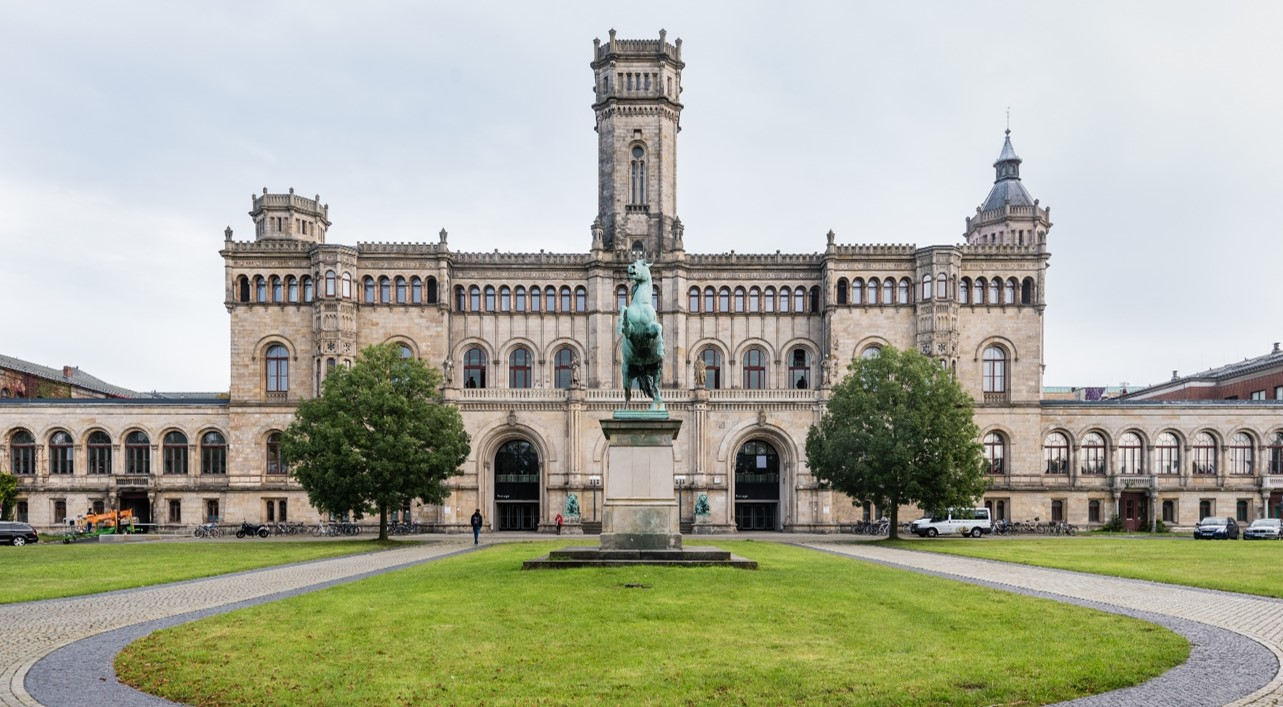
\includegraphics[width=0.65\textwidth]{figures/luh_default_presentation_title_image.jpg}}

% Title page: luhstyle
% \setbeamertemplate{title page}[luhstyle]
% % Add optional title image here
% \addtitlepageimage{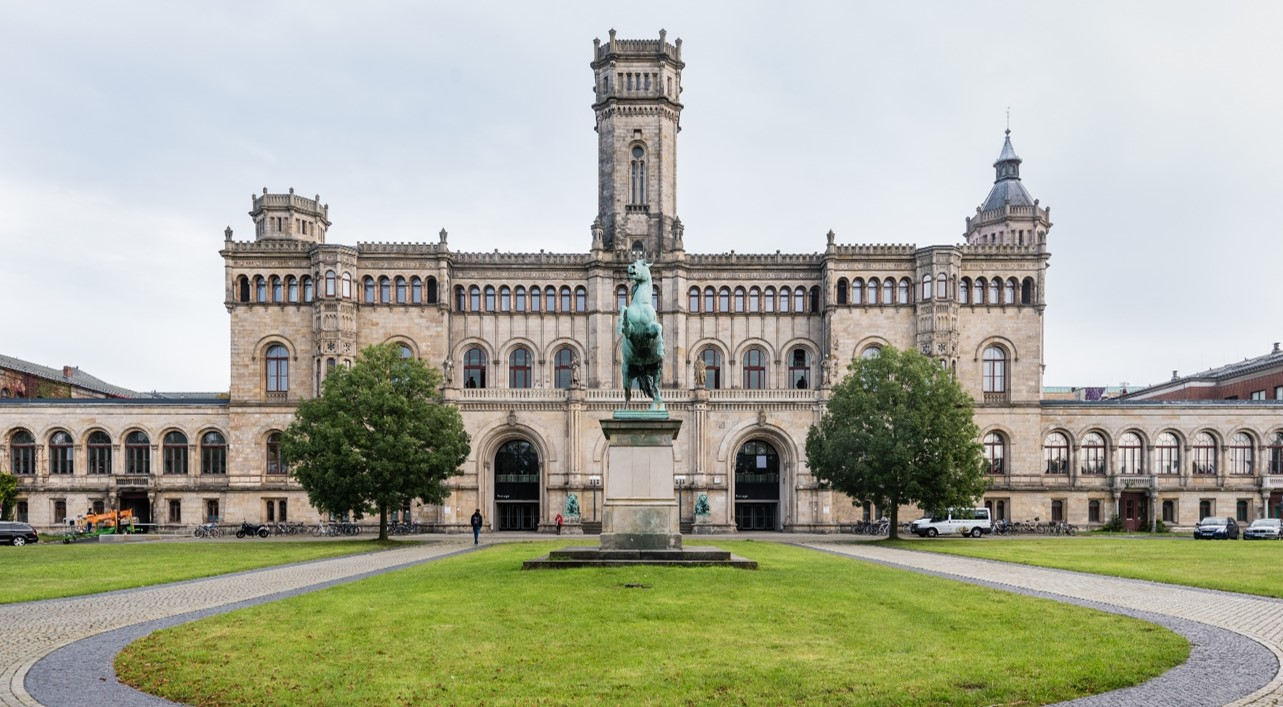
\includegraphics[width=0.75\textwidth]{figures/luh_default_presentation_title_image.jpg}}

\author[Abedjan \& Lindauer]{Ziawasch Abedjan \& \underline{Marius Lindauer}\\[1em]
	%
\includegraphics[height=\logoheight]{../latex_main/figures/luh_logo_rgb_0_80_155.pdf}\qquad
	
\includegraphics[height=\logoheight]{../latex_main/figures/DBIS_Kurzlogo.png}\qquad
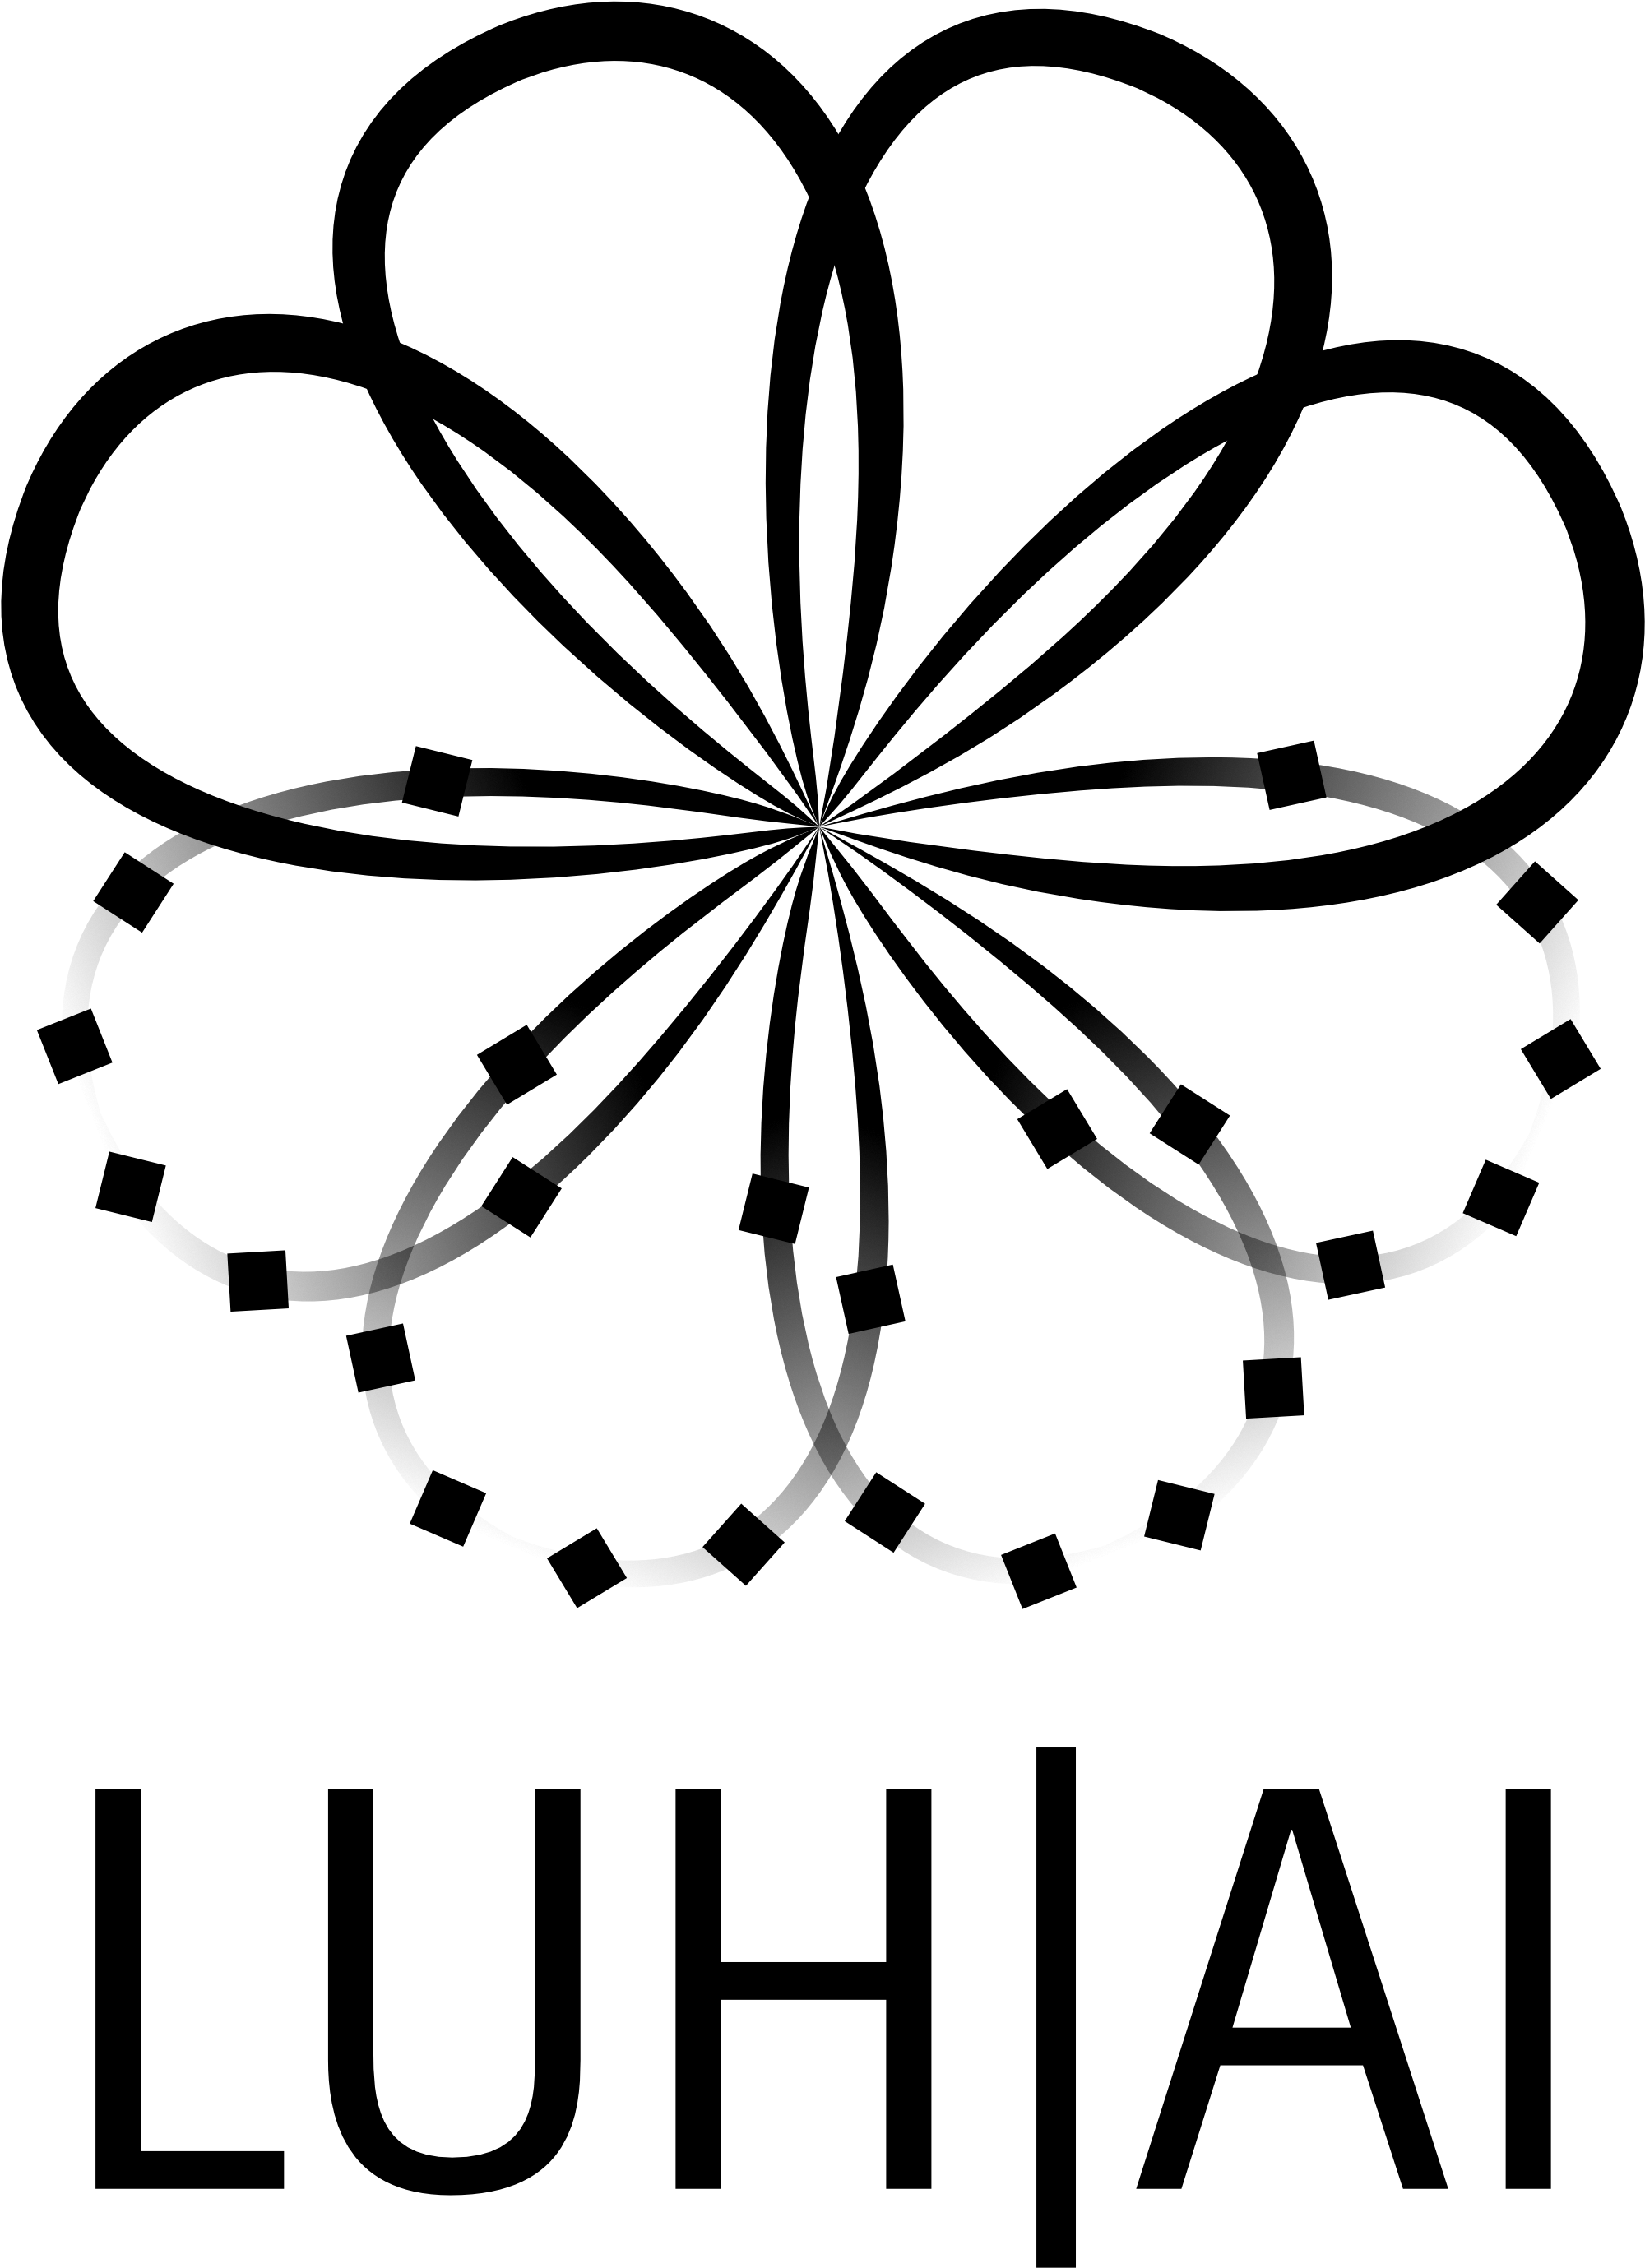
\includegraphics[height=\logoheight]{../latex_main/figures/logo_short_highres_black}\qquad

\includegraphics[height=\logoheight]{../latex_main/figures/Leibniz-AI-Academy_Logo}\qquad
%
\includegraphics[height=\logoheight]{../latex_main/figures/L3S.jpg}	
}
\date{\hspace{0.5em} {
\includegraphics[height=1.5em]{../latex_main/figures/Cc-by-nc-sa_icon.svg.png}}; extension of \href{https://ds100.org/fa21/}{[DS100]}
}


%%% Custom Packages
%----------------------------------------------------------------------
% Create dummy content
\usepackage{blindtext}

% Adds a frame with the current page layout. Just call \layout inside of a frame.
\usepackage{layout}


%%% Macros
%\renewcommand{\vec}[1]{\mathbf{#1}}
% \usepackage{bm}
%\let\vecb\bm

\title[Introduction]{DS: Decision Trees}
\subtitle{Decision Tree Basics}

\graphicspath{ {./figure_tree/} }
%\institute{}


\begin{document}

	\maketitle

	\begin{frame}{Decision Trees}
	    A Decision Tree is a very simple way to classify data. It is simply a tree of questions that must be answered in sequence to yield a predicted classification.
	    \begin{figure}
	        \centering
	        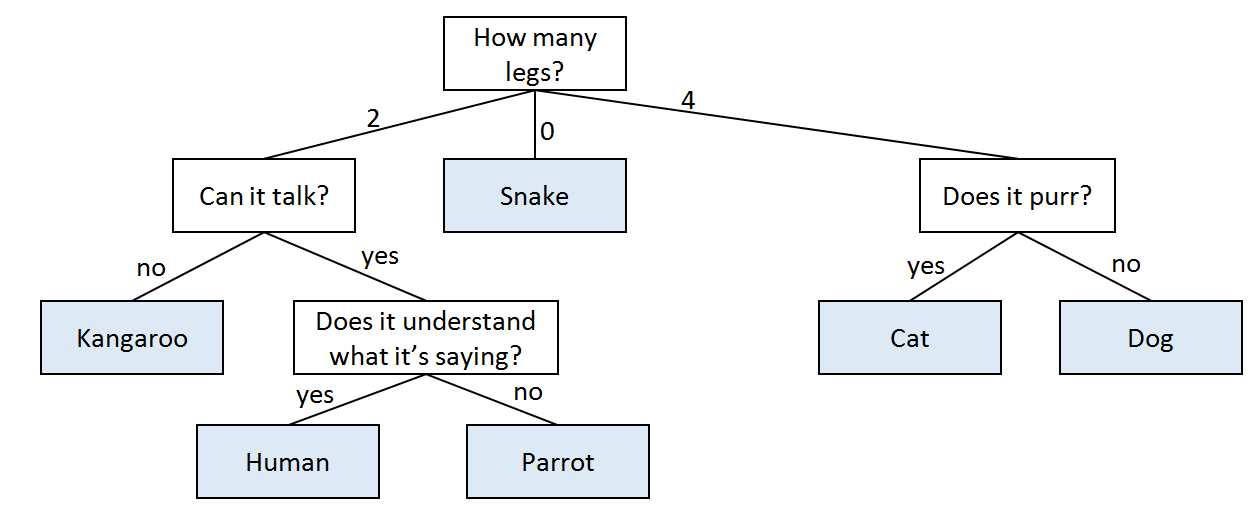
\includegraphics[scale=.35]{figure_tree/Bild1}
	    \end{figure}
	\end{frame}
 
	\begin{frame}{Example: Using Petal Data Only}
	    The plot below shows the width and length of the petals of each flower, with the species annotated in the form of color.\\
	    \bigskip
	    We can build a decision tree manually just by looking at this picture.
	        \centering
	        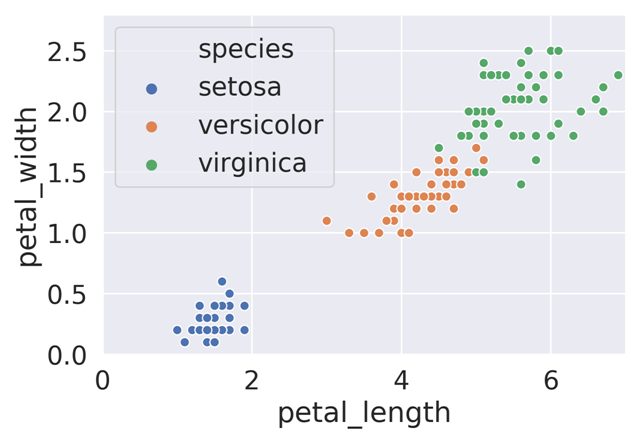
\includegraphics[scale=.65]{figure_tree/Bild3}

	\end{frame}
	
	\begin{frame}{Example: Using Petal Data Only}
	        %\centering
	        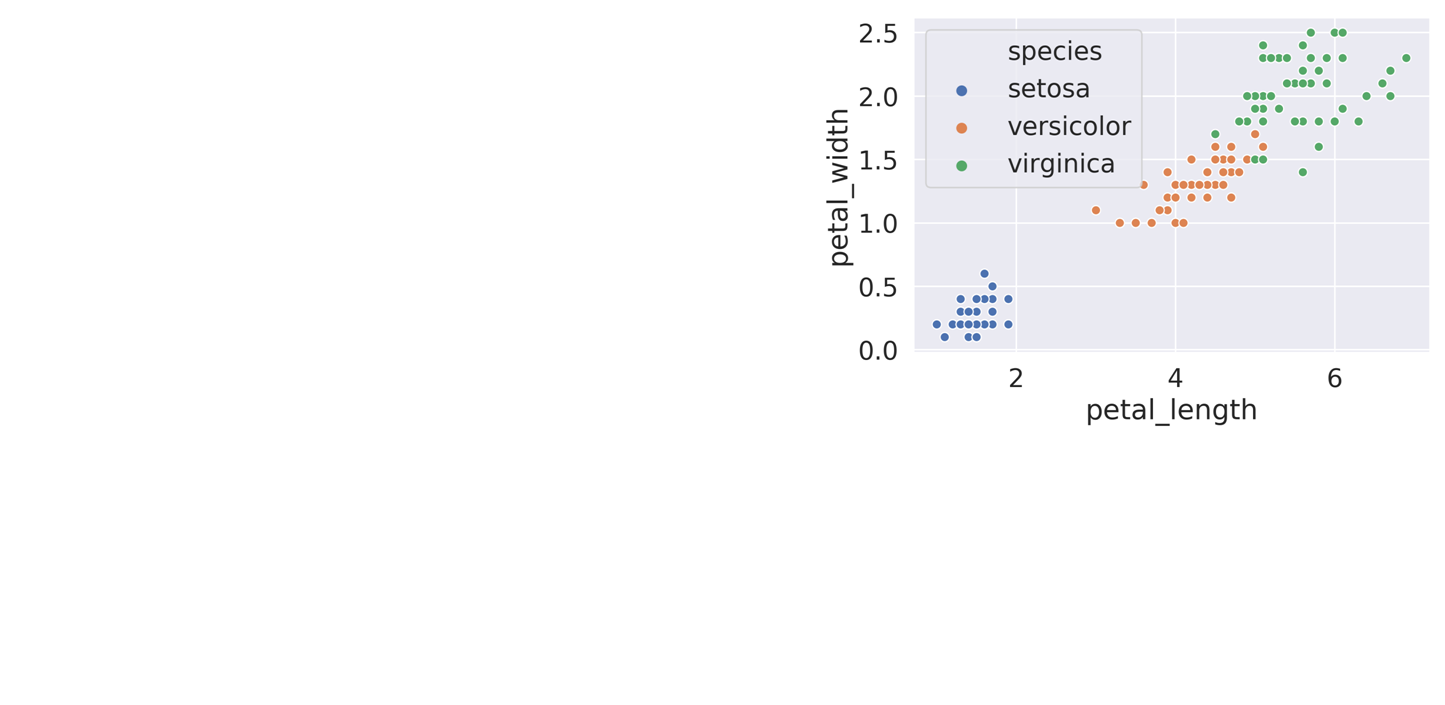
\includegraphics[scale=.34]{figure_tree/Bild5}
	\end{frame}
	
	
	\begin{frame}{Example: Using Petal Data Only}
	        %\centering
	        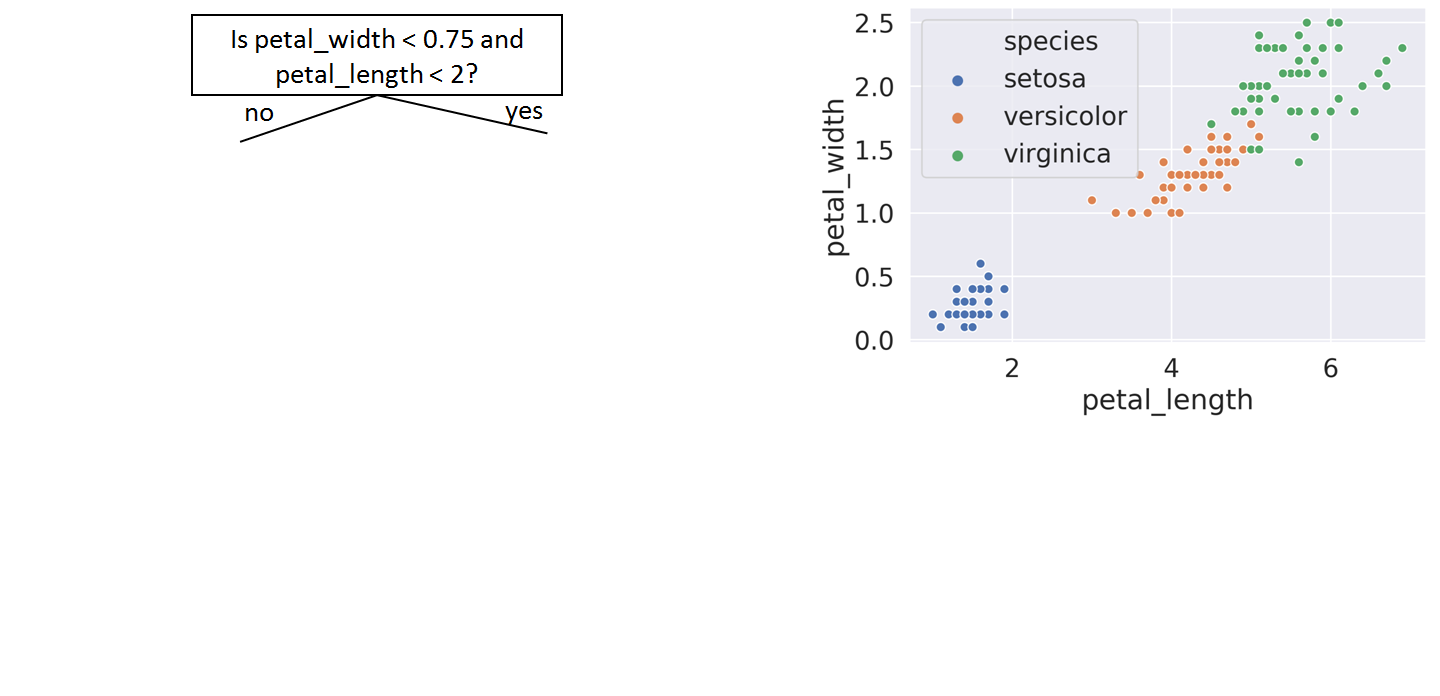
\includegraphics[scale=.34]{figure_tree/Bild6}
	\end{frame}
	
	
	\begin{frame}{Example: Using Petal Data Only}
	        %\centering
	        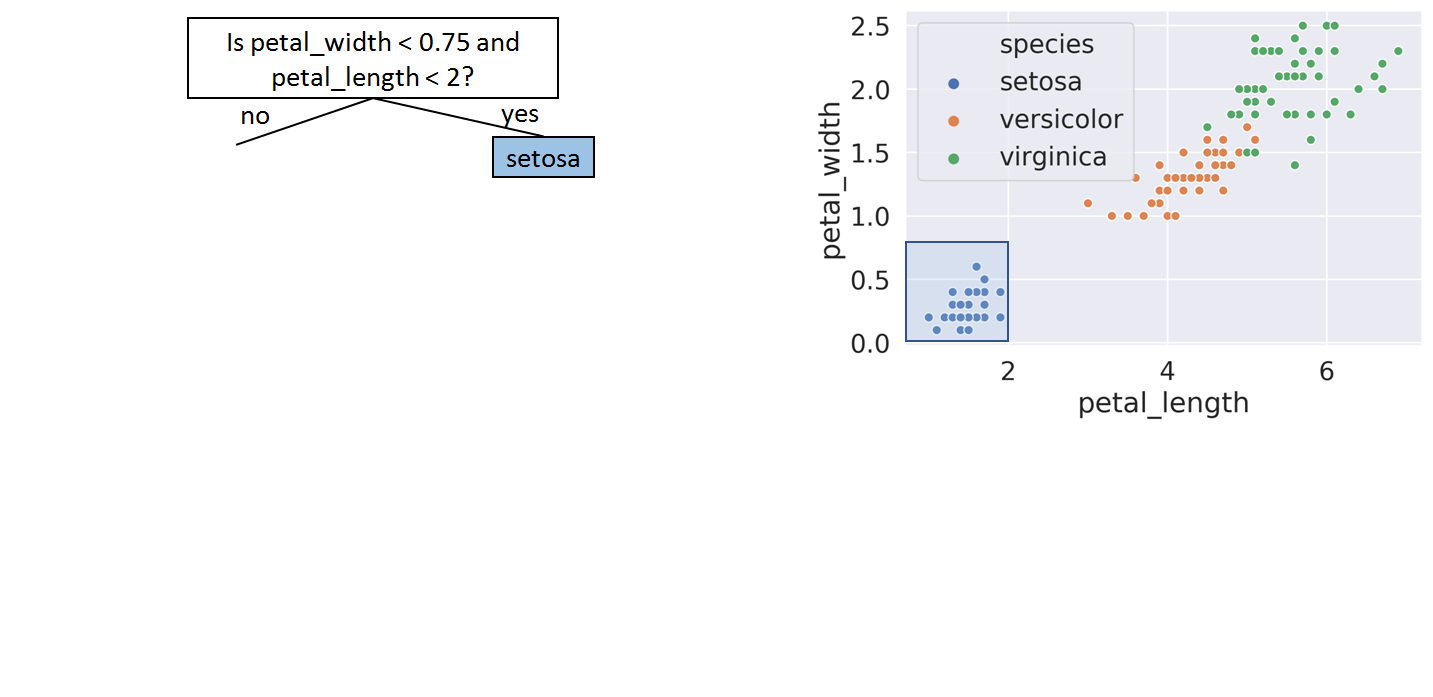
\includegraphics[scale=.34]{figure_tree/Bild7}
	\end{frame}
	
	
	\begin{frame}{Example: Using Petal Data Only}
	        %\centering
	        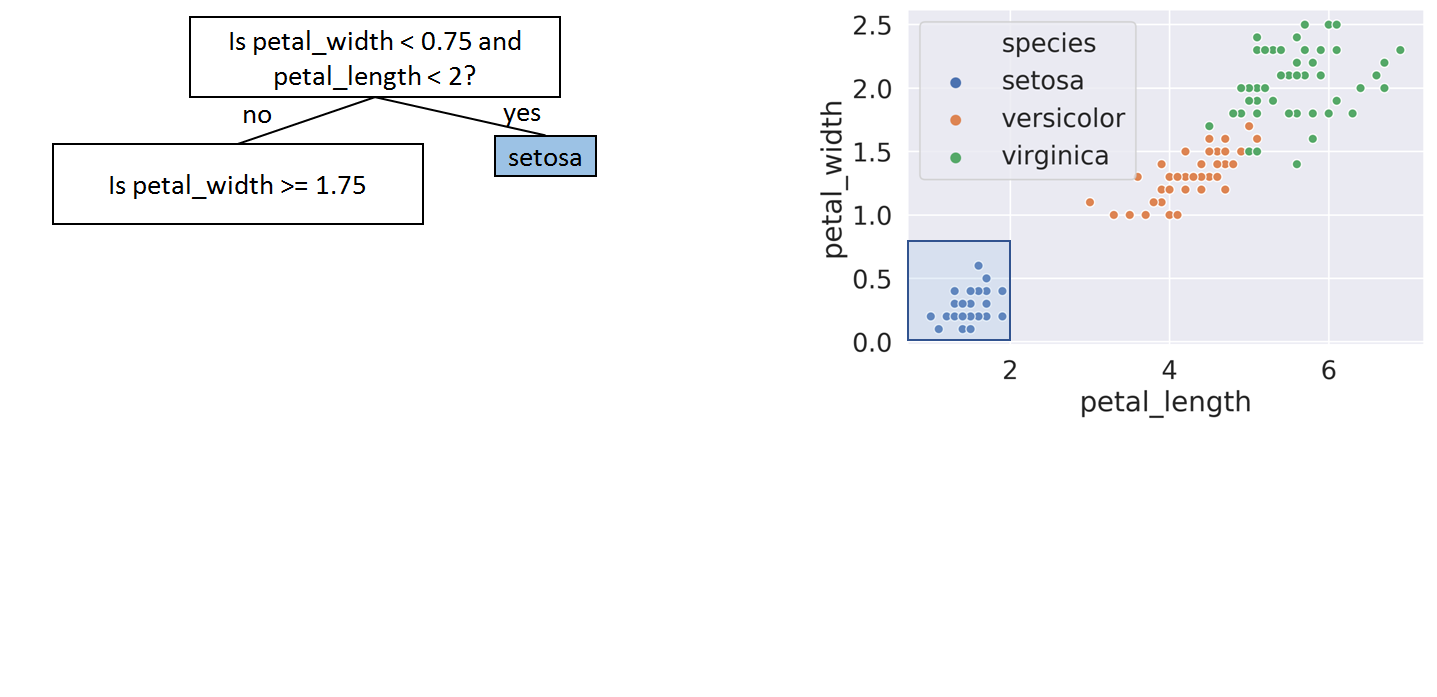
\includegraphics[scale=.34]{figure_tree/Bild8}
	\end{frame}
	
	
	\begin{frame}{Example: Using Petal Data Only}
	        %\centering
	        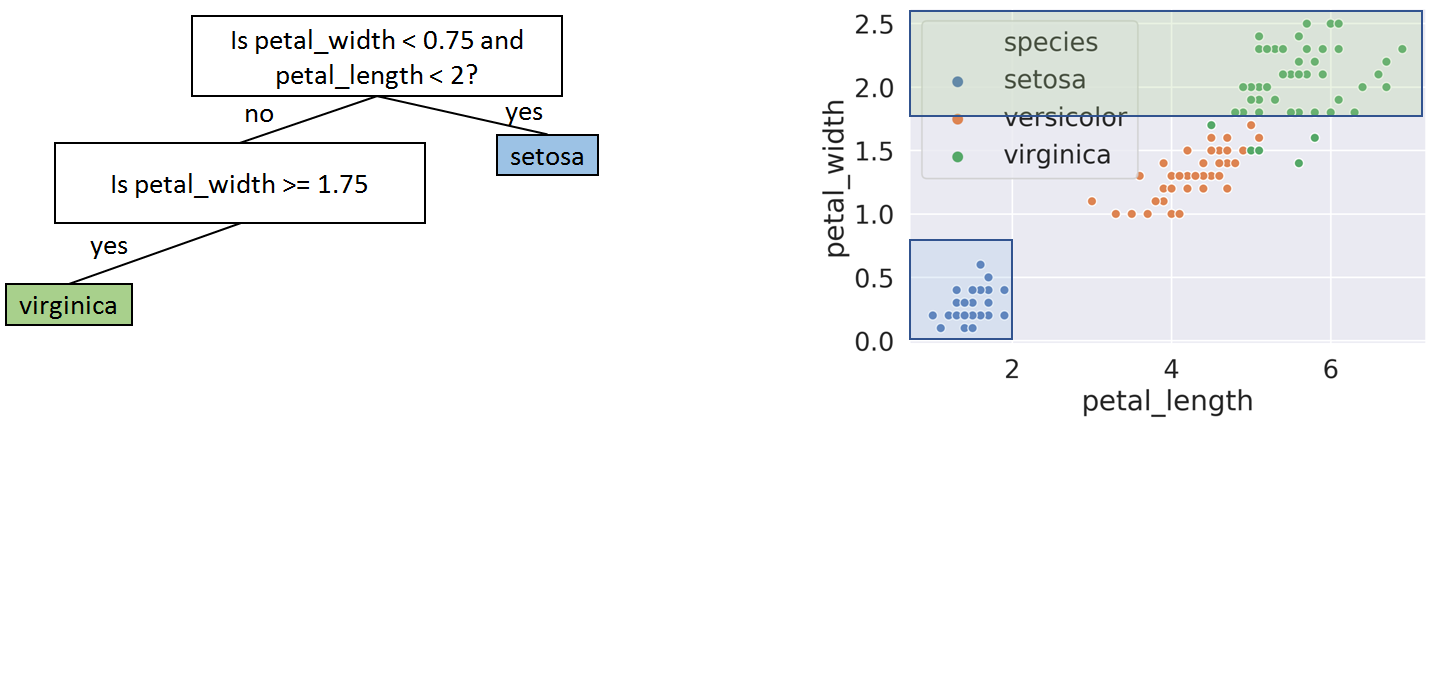
\includegraphics[scale=.34]{figure_tree/Bild9}
	\end{frame}
	
	
	\begin{frame}{Example: Using Petal Data Only}
	        %\centering
	        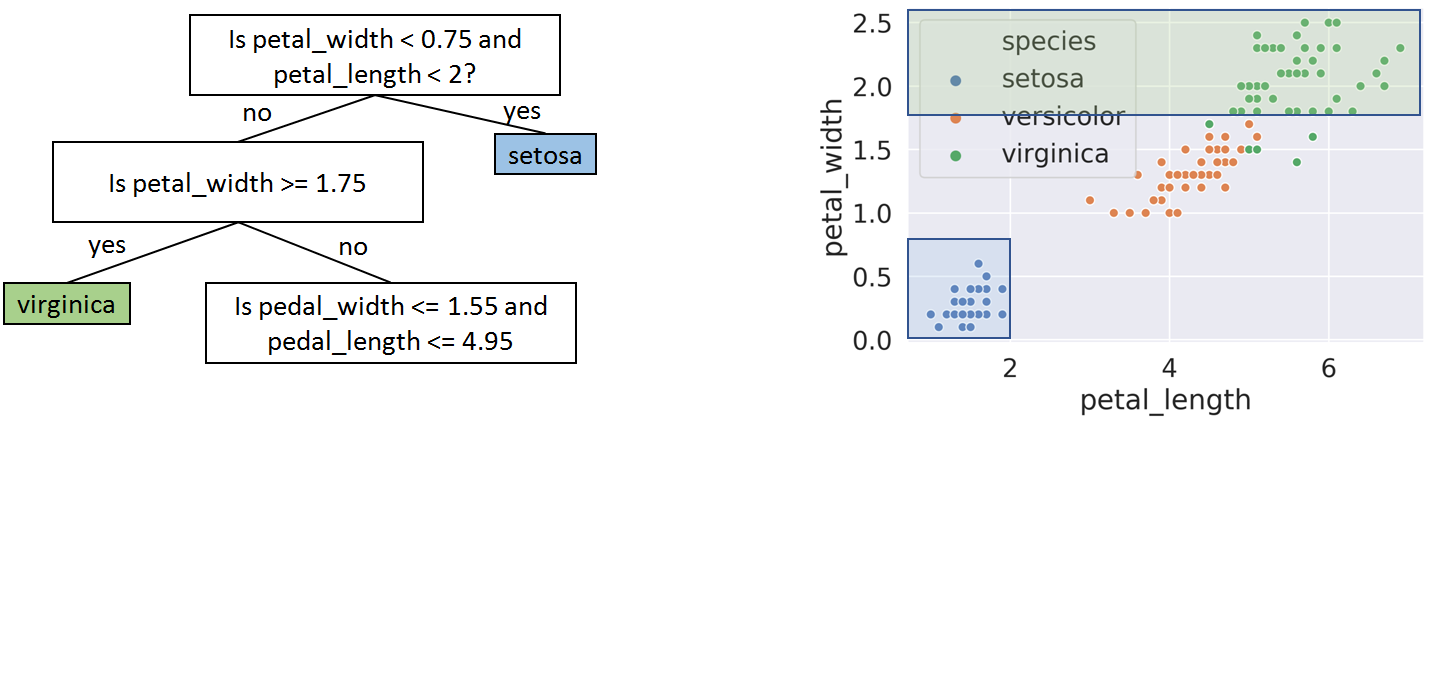
\includegraphics[scale=.34]{figure_tree/Bild10}
	\end{frame}
	
	
	\begin{frame}{Example: Using Petal Data Only}
	        %\centering
	        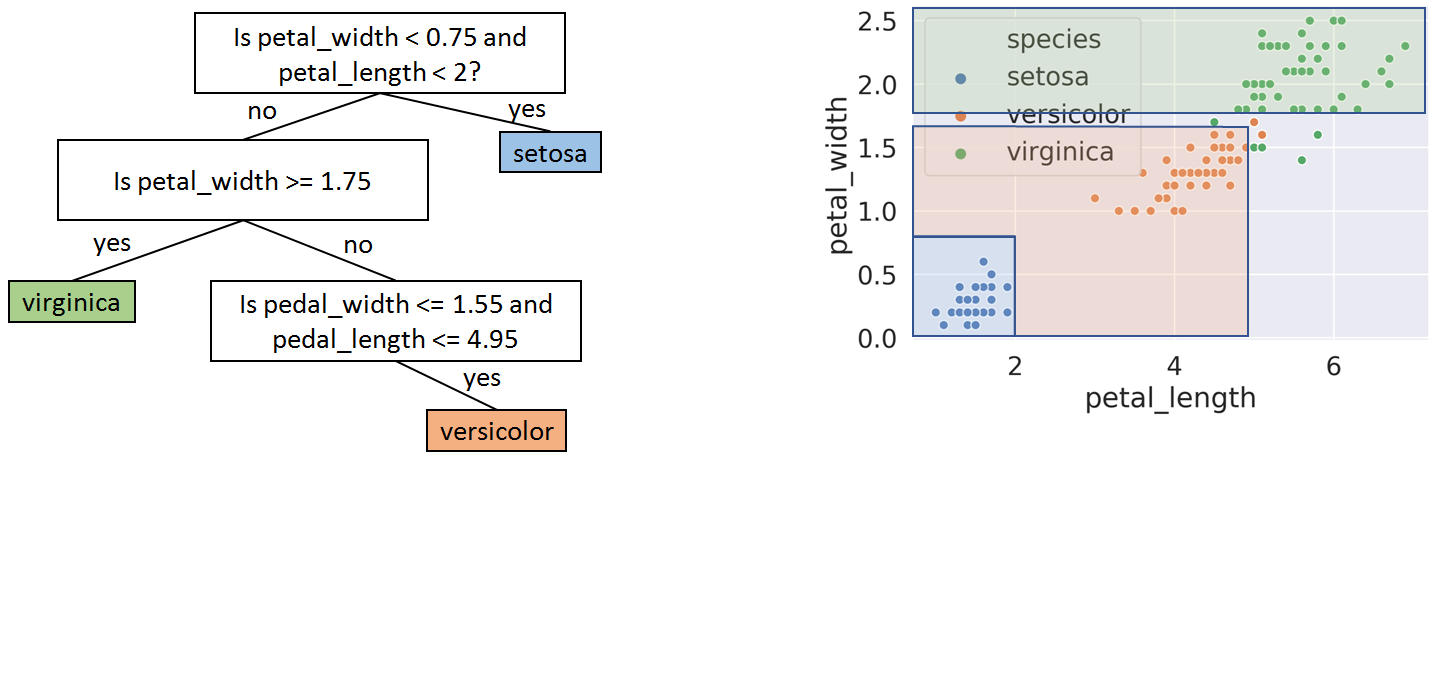
\includegraphics[scale=.34]{figure_tree/Bild11}
	\end{frame}
	
	
	\begin{frame}{Example: Using Petal Data Only}
	        %\centering
	        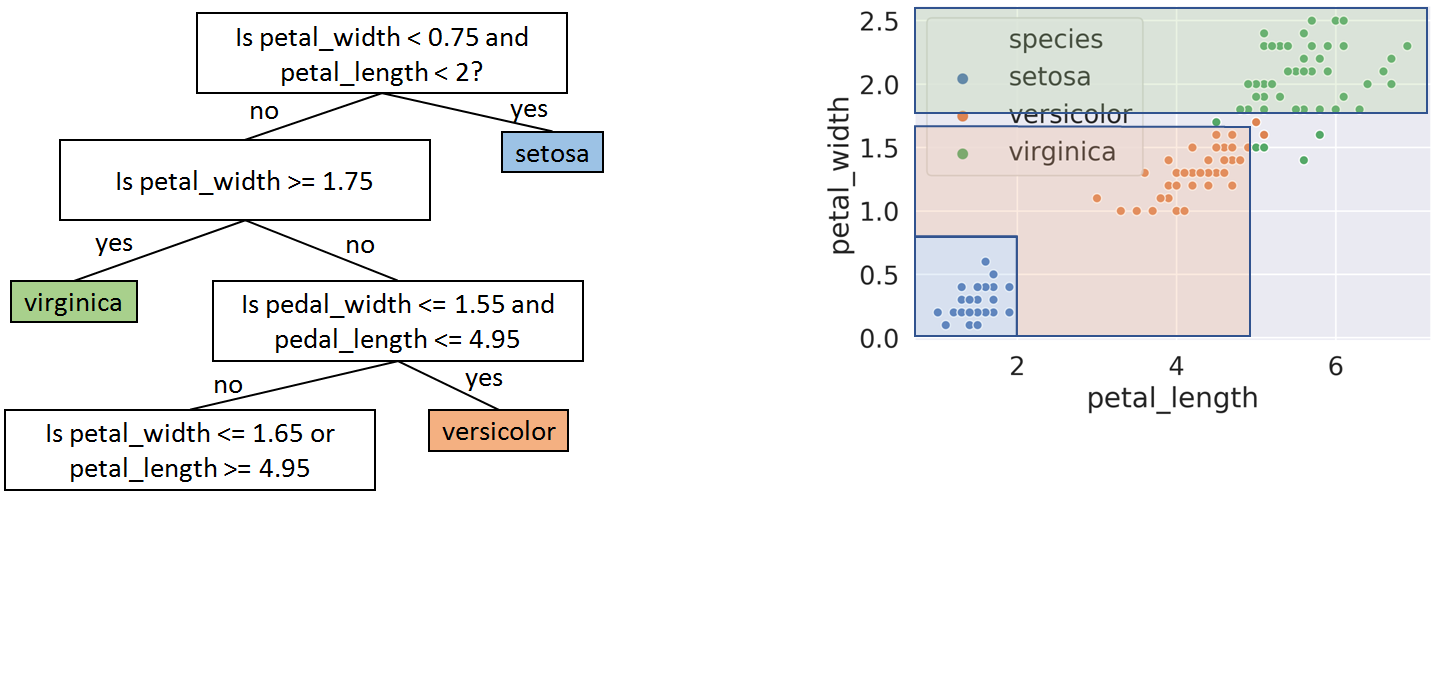
\includegraphics[scale=.34]{figure_tree/Bild12}
	\end{frame}
	
	
	\begin{frame}{Example: Using Petal Data Only}
	        %\centering
	        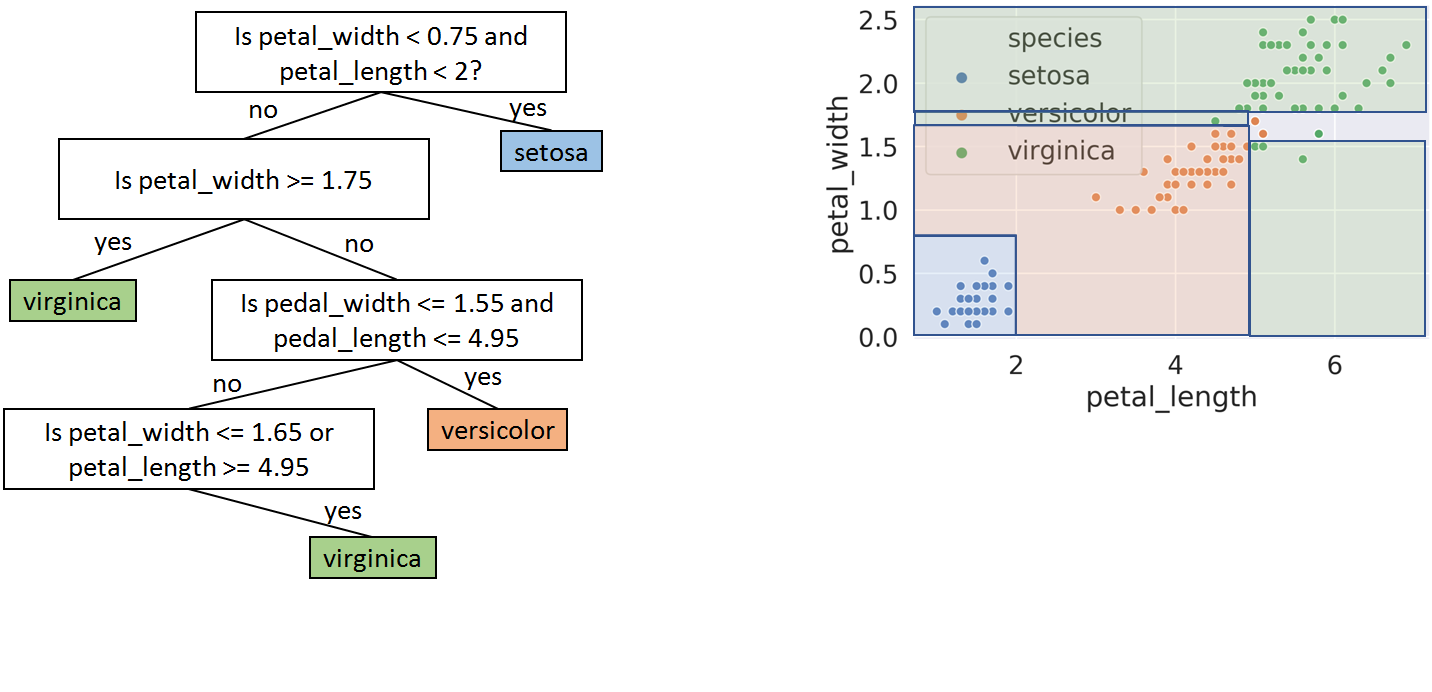
\includegraphics[scale=.34]{figure_tree/Bild13}
	\end{frame}
	
	
	\begin{frame}{Example: Using Petal Data Only}
	        %\centering
	        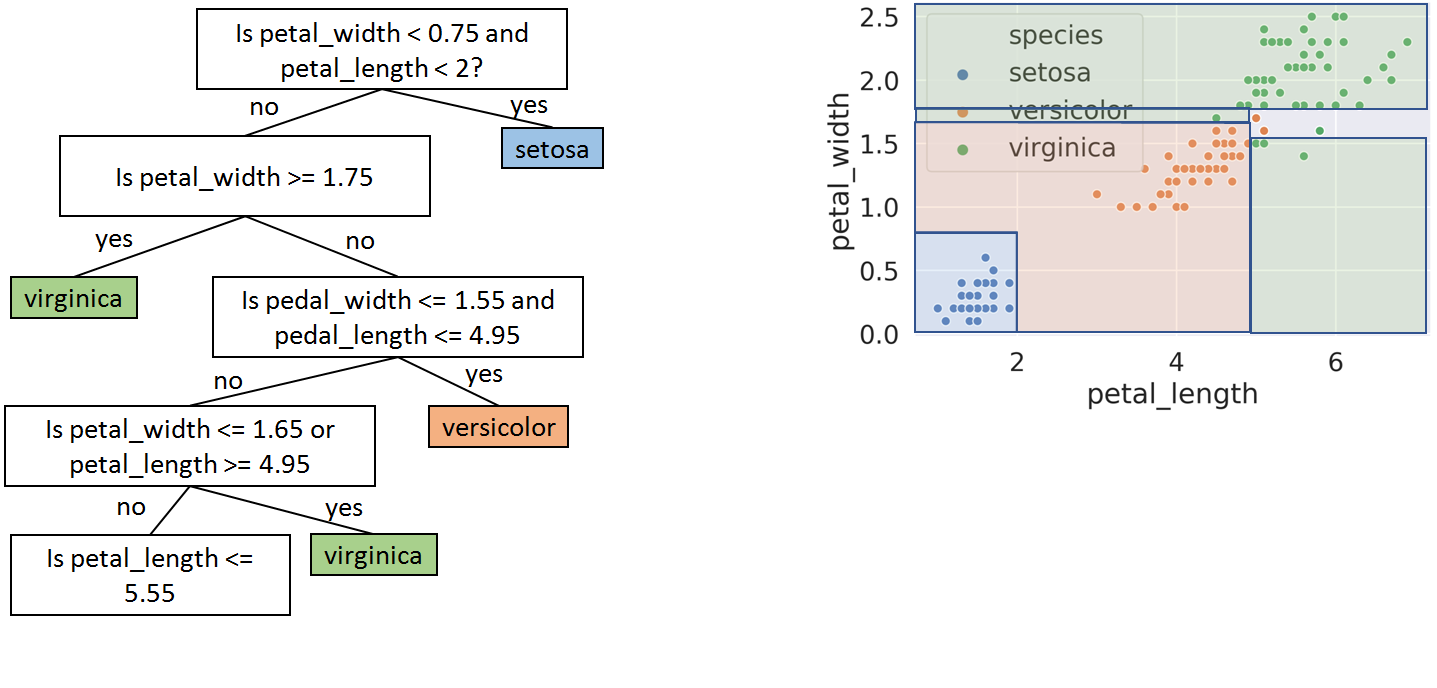
\includegraphics[scale=.34]{figure_tree/Bild14}
	\end{frame}
	
	
	\begin{frame}{Example: Using Petal Data Only}
	        %\centering
	        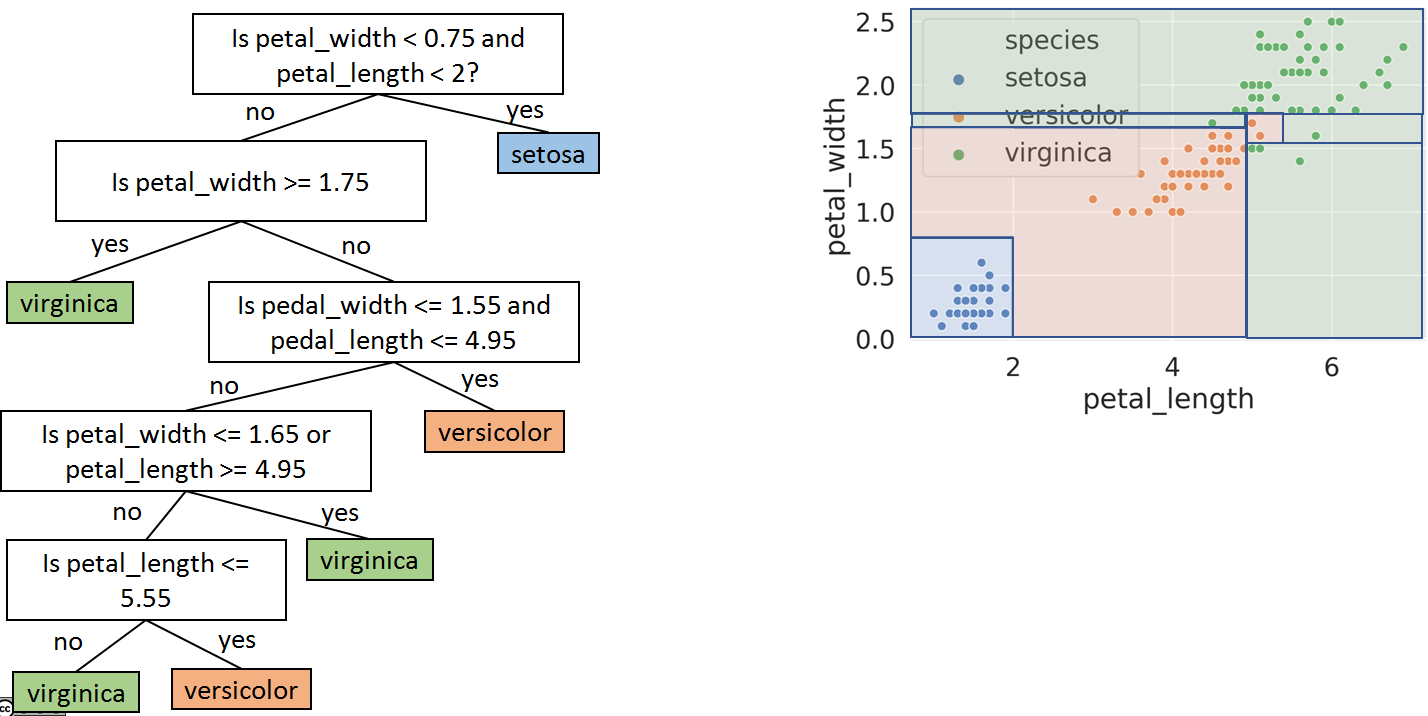
\includegraphics[scale=.34]{figure_tree/Bild15}
	\end{frame}
	
	
	\begin{frame}{Example: Using Petal Data Only}
	   \begin{columns}
	        \begin{column}{.5\textwidth}
	               How accurate is our decision tree model on the training data?\\
	               \bigskip
	                Is this good or bad?
	        \end{column}
	   
	   
	         \begin{column}{.5\textwidth}

	                    %\centering
	                     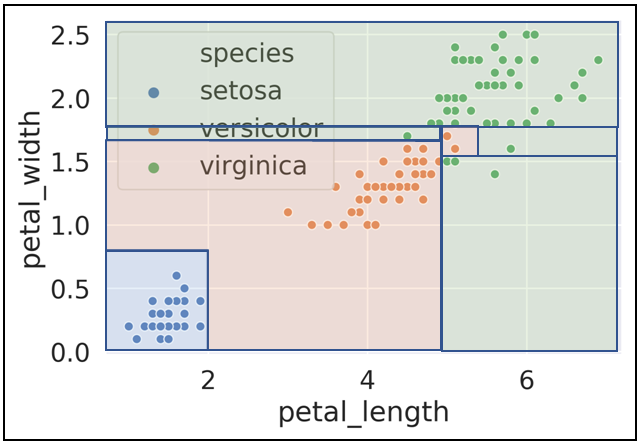
\includegraphics[scale=.34]{figure_tree/Bild16}

	        \end{column}
	   \end{columns}
	 \end{frame}
	 
	 
	 \begin{frame}{Example: Using Petal Data Only}
	   \begin{columns}
	        \begin{column}{.5\textwidth}
	        
	               How accurate is our decision tree model on the training data?\\
	               \begin{itemize}
	                   \item It seems like it gets every point correct
	               \end{itemize}
	               \bigskip
	                Is this good or bad?
	                \begin{itemize}
	                    \item Rather bad
	                    \item Seems likely to result in overfitting!
	                    \item Will discuss overfitting more later
	                \end{itemize}
	                
	        \end{column}
	   
	   
	         \begin{column}{.5\textwidth}

	                     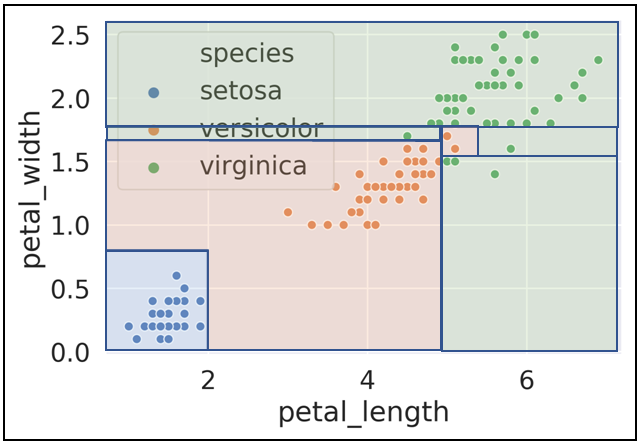
\includegraphics[scale=.34]{figure_tree/Bild16}
	                     
	        \end{column}
	   \end{columns}
	 \end{frame}
\end{document}